\section{Statik}
Generelles Vorgehen:
\begin{enumerate}[nosep]
	\item Skizze mit allen Kräften
	\item Koordinatensystem einführen
	\item Drehpunk von Drehmoment einführen
	\item Gleichgewichtsbedingung und Gleichungssystem aufstellen
	\item Gleichungssystem lösen
\end{enumerate}

~\\
\textbf{Beispiel Skizzen}

\begin{minipage}{\textwidth}	
	\begin{minipage}{0.25\textwidth}
		Haften:\\
		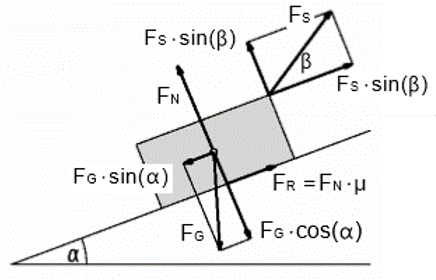
\includegraphics[width=\columnwidth]{./Images/Haften.png}
	\end{minipage}%%% to prevent a space
	\begin{minipage}{0.25\textwidth}
		Kippen\\
		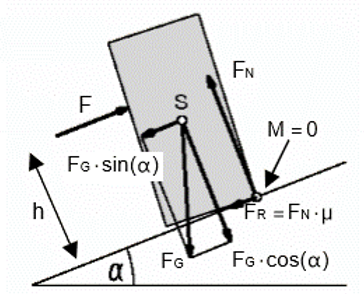
\includegraphics[width=\columnwidth]{./Images/Kippen.png}
	\end{minipage}
\end{minipage}



\subsection{Reibung \kuchling{104}}
\begin{formula}
	{F_R = F_N \cdot \mu} 
	
	F_R & Reibungskraft & [N] \\
	F_N & Normalkraft & [N] \\
	\mu & Koeffizient & [1]
\end{formula}
\noindent Der Haftreibungs-Koeffizient ist $\mu_H = \tan(\alpha)$ und der Gleitreibungskoeffizient $\mu_G= \tan(\alpha) - \frac{a}{g\cdot\cos(\alpha)}$. $\mu_h > \mu_g$

\subsection{Dichte}
\begin{formula}
	{\rho = \frac{m}{V}} 
	
	\rho & Dichte & [kg/m^3] \\
	m &    Druck & [N/m^2] \\
	V &    Volumen & [m^3]
\end{formula}

\subsection{Dehnung \kuchling{184}}
\begin{formula}
	{\sigma = \frac{F}{A} \\ = E \frac{\Delta l}{l}	= E\varepsilon}
	
	\varepsilon & Relative Längenänd. & [m]\\
	l & Länge \underline{ohne} Kraft & [m]\\
	\Delta l & Längeänd. \underline{mit} Kraft & [m]\\
	E & Elastizitätmodul & \\
	\sigma & Druck & [N/m^2]\\
	A & Querschnittsfläche & [m^2]\\
\end{formula}

Für Elastizitätmodul $E$ siehe \kuchling{624}

\subsection{Druck/Spannung}
\todo{}
\begin{formula}
	{\sigma = \frac{F_\perp}{A}} 
	
	\sigma & Druck & [N/m^2]\\
	...
\end{formula}
\begin{formula}
	{\tau = \frac{F_\parallel}{A}} 
	
	\tau & Schubspannung & [N/m^2]\\
	...
\end{formula}